

\section{Implementation Overview}

In this work a cloud simulation framework has been established to be able to assess the outcome of different scenarios in a defined setting. The goal was to deliver a complete framework that can handle multiple data sources and is extendable for future work with possibly different data sets and an optional connection to a real cloud environment which could replace the simulated cloud environment that is connected to the framework in this implementation. 

The implementation consists of three parts which will be presented separately below. The first part represents the data handling and management interfaces implemented on a Java Application Server connected to an Oracle database. The purpose of this platform is to have a generic means of parsing and fetching data from various sources that can be defined in advance. For example, data may be fetched from local files that were previously retrieved from energy markets or remote web services that provide energy data of that respective energy market. In addition parsers for different file formats may be defined to automatically parse data and put it into the database for later retrieval. From there arbitrary queries may be executed to retrieve and aggregate data in a specific fashion and execute further tasks based on that data. 

The second part consists of a collection of statistical methods that should assist in making accurate forecasts based on the previously collected data. Through these methods sophisticated analysis can be executed to examine various datasets and apply customized models to each of these datasets. The purpose behind these statistical examinations is to provide meaningful and accurate forecasting models that can be utilized by the simulation framework. Eventually the performance of forecasts within the simulation should be examined and compared with approaches based solely on currently available data. It is expected that the application of accurate forecasts to energy price time series within the simulation improves overall performance and thus further energy cost savings are possible. 

The third part constitutes the actual cloud simulation which is based on a previously existing and sophisticated cloud simulator written in Python that incorporates cost models for energy and cooling expenses and is easily extendable by integrating custom schedulers. In this work custom settings have been applied to allow for a simulation that meets the needs of the framework to integrate different scenarios. Various parts of the simulator needed to be extended and a completely new scheduler has been built to schedule both cost aware and non-cost aware scenarios. It works together well with other parts of the framework s.t.~it is possible that live retrieval of data and forecasts are made from the application server through well defined interfaces. The components are decoupled such that each of them may be replaced by other components easily provided that the same interfaces are offered. 

This chapter is divided into an architectural section with an architectural outline followed by a section about statistical model selection and tools and a detailed presentation of the simulator and scheduler that actually run through the simulation scenarios. Then the results from the simulation runs based on different settings and data is presented and scenarios are compared to evaluate the most promising approach in the defined setting. Finally the results are discussed and evaluated to draw conclusions about the possible performance gains when running these scenarios, and how much they differ from the optimal solution. 


\section{Architectural outline}

The architectural outline provides an overview of all components involved in the presented simulation framework and how they work together. All components may interact with one another via defined interfaces s.t.~either component may be replaced by a similar component with possibly different implementation details but same interfaces. 

\begin{figure}[htbp]
	\centering
		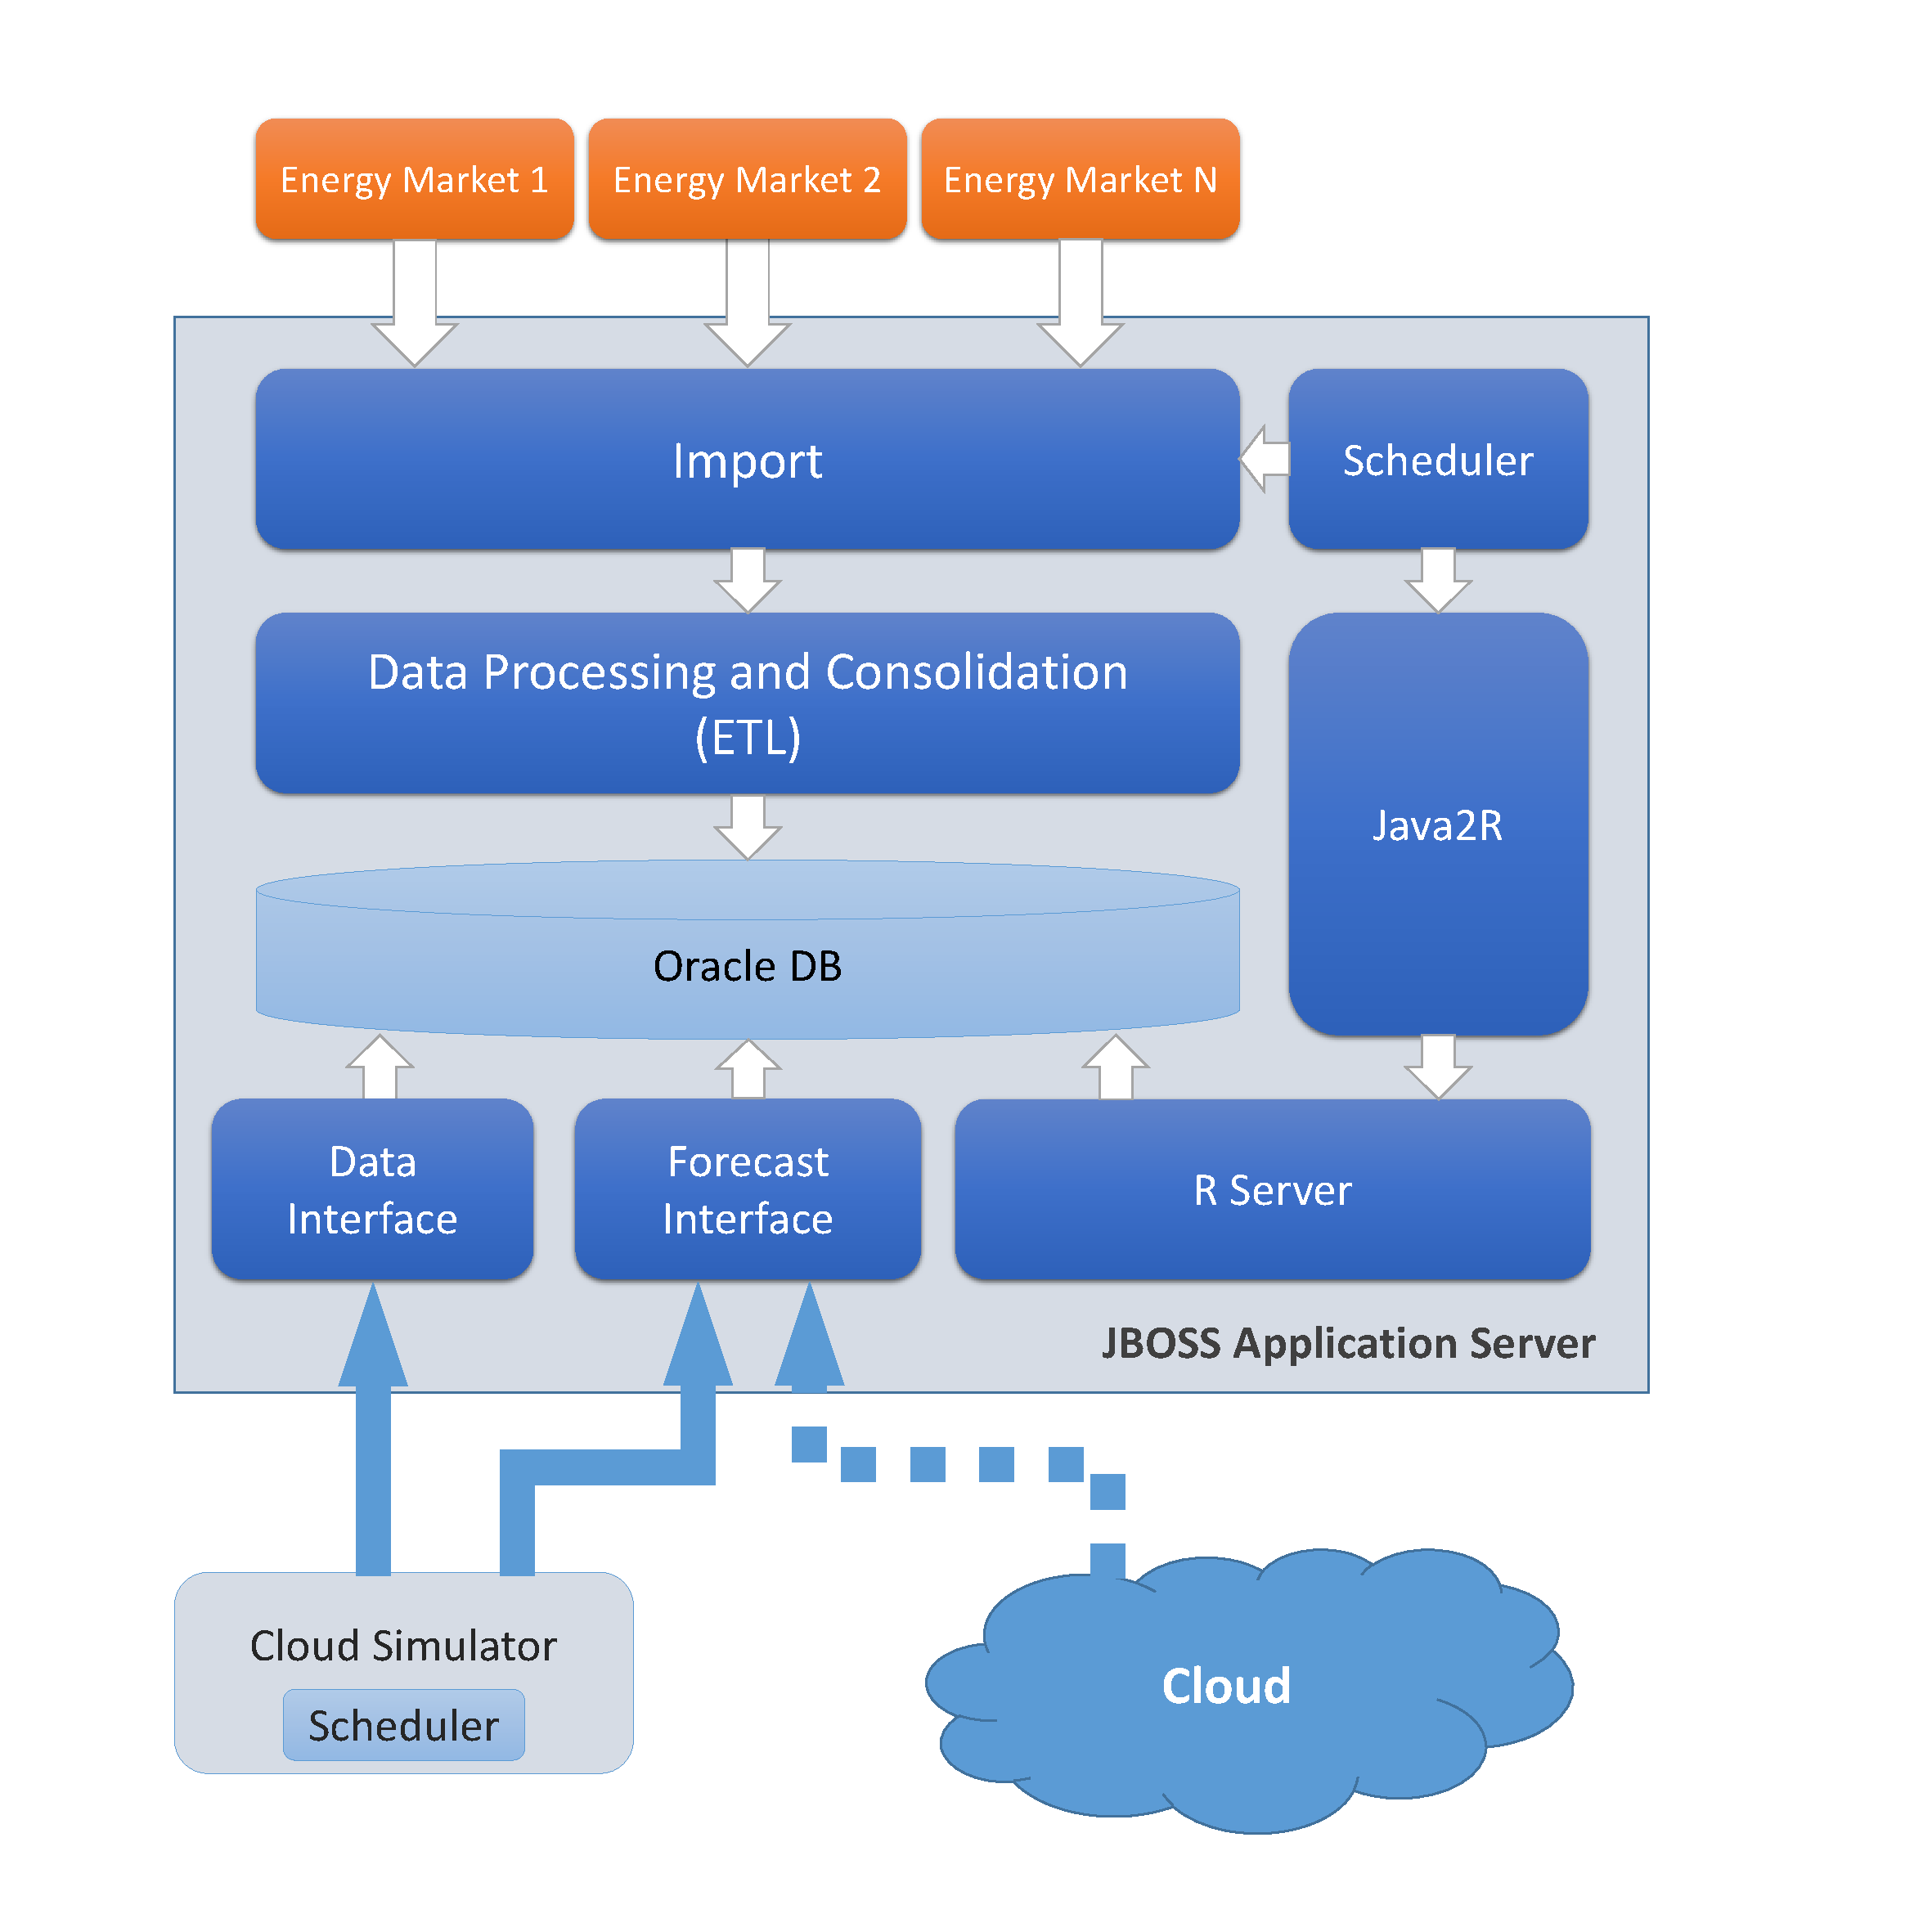
\includegraphics[width=0.9\textwidth]{../../docs/architecture/Block_Diagram_Architecture.pdf}
	\caption{Architecture Block Diagram}
	\label{fig:Block_Diagram_Architecture}
\end{figure}

Figure \ref{fig:Block_Diagram_Architecture} depicts a block diagram of the simulation framework that shows which components are included and how they interact with one another. Data retrieval from the energy markets is done by the import module as the first action in the process. Several energy markets and their interfaces may be registered beforehand to retrieve data from these interfaces. The scheduler triggers the import at a defined time interval (e.g.~every hour or once per day). 

From the import module the retrieved data is handed over to the Data Processing and Consolidation module which transforms the data to a common format such that it can be fed to the database. This process is similar to the well known ETL process (Extract Transform Load) which extracts data from various sources, transforms it into a defined data format and loads it into a data warehouse or database. The applied process in this work is similar as parsers for different file formats exist that can be configured to parse data from different sources. After the data transformation process the retrieved energy prices are stored in the database from where they can be further processed. 

The scheduler component is also responsible for triggering the generation of R models where the respective interface for model generation is called. The Java2R interface provides a means of calling methods on the R server that analyzes the data and generates the models. As the generation of forecasting models can take a considerable amount of time depending on the amount of data provided to the model this mechanism ensures that model generation is done as soon as data is available to have it available when it is needed. 

The R server does not directly connect to the database but saves the binary models in the file system of the application server. From there it can be retrieved easily by forecasting interfaces that are based on the generated models. The reason the models are saved in the file system is because they are frequently generated and are outdated when new data is available. Therefore file system access is easier and faster as these models typically are only of temporary importance and may be overwritten by subsequent models. 

The data and forecast interfaces are a means of providing data to external components such as the simulator or a real cloud. The data interface provides historical data to be retrieved from different energy markets and locations as well as time stamps for the purpose of getting customized data for simulations. The forecast interface provides a convenient way of retrieving forecast data for specific locations and time ranges. As model generation already happened beforehand the forecasts can be provided instantly also for historical data for simulation purposes. It is possible for a real cloud environment to use the forecast as well as the data interfaces to incorporate the data into the existing workflow. 


\subsection{Components and Interfaces}

In this section a more detailed view on the various components of the framework is provided and the interfaces that exist between them. Figure \ref{fig:Component_Diagram} shows this view in form of a component diagram. 

\begin{figure}[htbp]
	% used to position the image at the horizontal center of the page
	\hspace*{-0.4in}
		% include the graphic rotated by a 90 degree angle and scale to paperwidth and height
		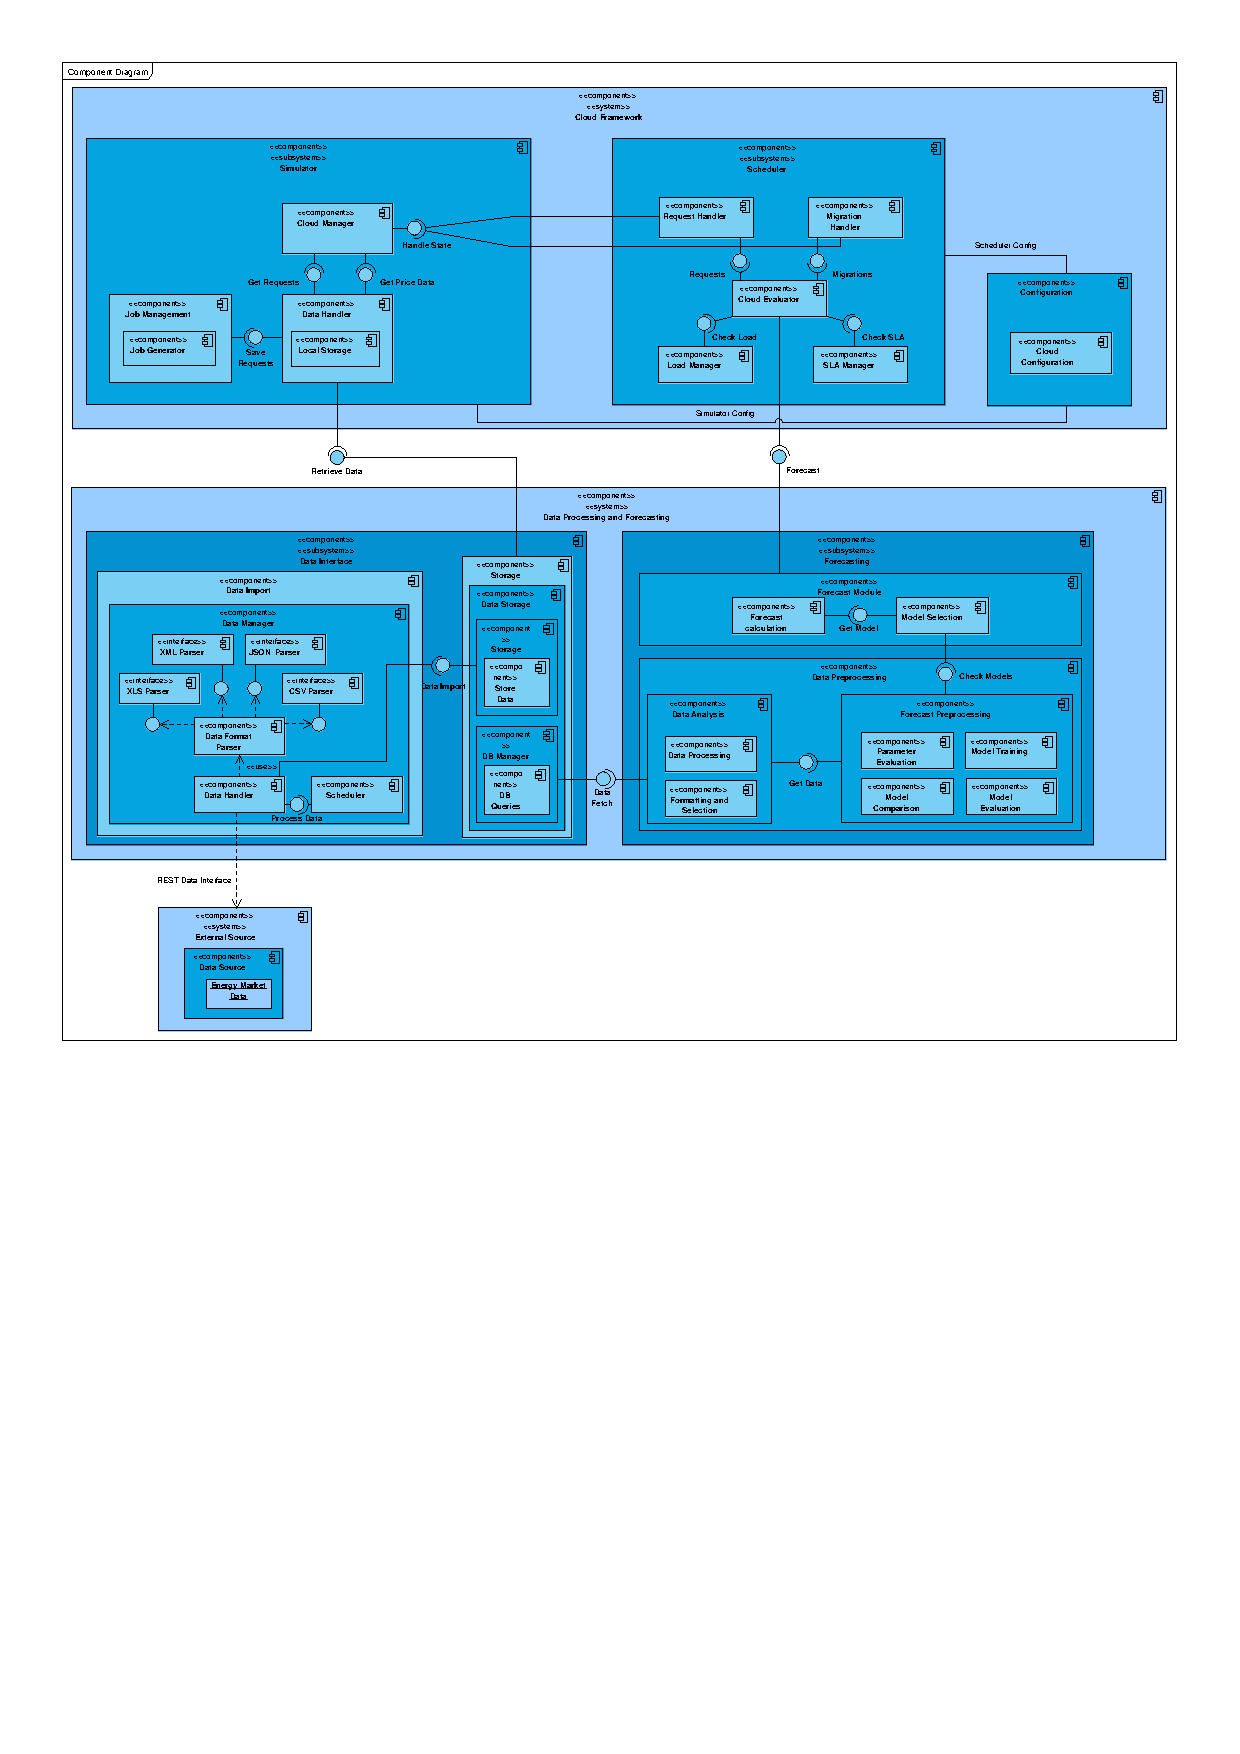
\includegraphics[angle=90,width=\paperheight,height=\paperwidth,keepaspectratio=true]{../../docs/architecture/UML/Component_Diagram.pdf}
	\caption{Component Diagram}
	\label{fig:Component_Diagram}
\end{figure}

The diagram consists basically of two parts, the Cloud Framework and Data Processing and Forecasting. The Data Processing and Forecasting part consists of the Data Interface and Forecasting components that are responsible for data import and retrieval and forecast model generation. The Cloud Framework contains the cloud simulator and scheduler which are responsible for the actual simulation and application of scheduling algorithms. It is also used to generate the resulting time series, e.g.~cloud utilization and energy cost over time. 

The Data Interface component retrieves data from previously registered energy markets as indicated by the dashed line connection to the external data source. The data imports are triggered by the scheduler which calls the respective services at the Data Handler. The Data Handler uses appropriate parsers to extract data into a common data format. When data processing is finished the Data Import for storing the data into the database is called from where it can be retrieved via DB Query components. The DB Queries are used by the Forecasting component to retrieve data for model evaluation and generation. 

The Forecasting component fetches data from the database and does some data preprocessing that is used for forecasting. After the data has been processed and formatted appropriately it is then ready to be analyzed by statistical methods to determine which forecasting model suits best for the selected time series. Different models are trained and compared and the best model is chosen. It is then selected by the Forecast Module and the actual forecasts are calculated which can be queried via a provided public interface that is exposed to external systems. 

The Cloud Framework uses the historical price data provided by the Data Interface component to run simulations for various scenarios. It is read into a local storage for further processing of the price data in simulations. Job requests are generated that reflect certain characteristics or requirements of tasks that should be processed by the Cloud Framework. Requests and energy prices are read by the Cloud Manager that keeps track of the cloud's current state. The state is retrieved and modified by the scheduler that handles requests and possible needs for migrations. At each step the Cloud Evaluator gets current request and migration demands and checks if load and SLA constraints are met. If that is the case the resources are moved to the respective server. Both scheduler and simulator components are configurable by a config file defined by the Cloud Configuration component. Thus new configuration options are easily added and can be changed at any time to adjust the output of simulations. 


\subsection{Application Server}

Considering the need for easy and generic data handling when dealing with different energy markets and data formats the application server has been set up which is connected to a database to fetch and parse data for later processing. By this means it is possible to execute extended data analysis tasks and aggregate and combine data to get insights into possible relationships between different data sets. Scenarios based on different datasets are easily created to quickly run simulations under changing conditions. Thus it is a flexible way of data handling that also simplifies the whole simulation process. 

Another benefit of providing an application server is the possibility to expose web service interfaces that can be called by any external component to utilize data and forecast interfaces. The architecture has been made extensible such that a new energy market location can be added without touching existing interfaces. 
Data processing interfaces exist for different data formats which can be extended to provide implementations for different energy price data. 

\subsubsection{Data management}

Interfaces for data management are defined within specialized Java classes that are responsible for the retrieval, import and data query handling. 

\subsubsection{Web Services}

All publicly exposed interfaces are designed as web services that can be called by any application regardless of its type or implementation. Specifically REST service interfaces have been chosen as it is a simple yet powerful method of providing reliable interfaces for interactions with the server. The underlying Java technology is JAX-RS which is a common implementation for providing REST service interfaces on Java application servers. Data may be passed by Path or Query parameters that are specified at each service interface. 

\subsubsection{Scheduling}

The application server also includes scheduling services where actions are triggered at each interval. This relates to the continuous and automatic import of data from various energy markets and the subsequent generation of R models. Therefore at each service invocation the respective REST interfaces are called to import the latest data from the markets and trigger the model generation based on that data. This mechanism allows for statistical models to be always up to date and are saved and retrieved based on the last date of the underlying trainings data. 




\subsection{Simulator and Scheduler}

\subsubsection{Basic structure}

\subsubsection{Configuration}

\subsubsection{External interfaces}

\subsubsection{Scheduler}


\subsection{R Server}

R is a statistical tool with vast amounts of statistical methods for data analysis and model generation\footnote{\url{https://www.r-project.org/}}. It has been chosen as the statistics engine for this work since it does not require a commercial license and became the de-facto standard for statistical processing over the last decade. 

\subsubsection{Forecast Models}

\subsubsection{Assessment of Forecasts}

\subsubsection{Forecast error evaluation}


\subsection{Database Server}

\subsubsection{Schema outline}

\subsubsection{Entities}

\subsubsection{Application server interface}



% Scheduler Types

% Benefits and drawbacks
 
% Settings and configuration



%\section{Cloud-based Simulator}

%\subsection{Motivation}
%
%\subsection{Structure of simulator}
%
%\subsection{Functional requirements}
%
%%TODO 
%Discuss impact of evaluation of bandwidth costs. In \cite{rao2010minimizing} %(page 7) 
%bandwidth costs are deliberately neglected, but the option should be still taken into account. As these costs directly relate to costs of migrations it is vital to include and model them within the scenarios. 
%
%\subsection{Non-functional requirements}
%
%\subsection{Incorporating forecast models}
%
%As already discussed in the introduction %TODO WHERE ?(forecast chapter? TODO) 
%forecasting is an integral component of the simulation as it should support in decision making when assigning workload and performing migrations. Since forecast errors can have a negative impact on workload allocation which may result in non-optimal workload distributions \cite{de2013study} it is of paramount importance that the forecast models are trained thoroughly and forecast errors are kept at a minimum. In order to reduce the impact of forecast errors in the simulation forecasting is done several hours into the future whereby the results are averaged to obtain a broader estimate of energy prices of the near future. 



\section{Model selection}

\subsection{Model type selection}

\subsection{Model selection based on data}

\subsection{Accuracy of selected models}


\section{Simulation and Scheduling}

\subsection{Cloud settings}

\subsection{Cost models}


Cost models are required to map the servers' energy consumption to costs depending on current energy prices. Different cost models exist exhibiting higher or lower accuracy and differ in their type of calculation. 

In this thesis several assumptions have been made: 

\begin{itemize}

\item \textbf{idle power.} A server has a defined idle power (e.g.~100 Watts (W)). This is the power that is drawn when the server is in idle mode (no tasks are running). 

\item \textbf{peak power.} A server has a defined peak power (e.g.~200 Watts (W)). This is the power that is drawn when the server runs on maximum load (maximum number of tasks running). 

\item \textbf{utilization.} Each server has a utilization between 0 and 100 percent. A utilization of zero percent means the server is idle, in contrast a utilization of hundred percent means the server is at peak load. 

\item \textbf{power consumption.} The power consumption is defined as the effective power consumed by a server during a certain period of time (e.g.~one hour). The result is a measure of power consumed per time (e.g.~150 Watt hours (Wh) for a server running on 50\% utilization for one hour)\footnote{\url{http://whatis.techtarget.com/definition/kilowatt-hour-kWh}}. %Energy can also be measured in Joule (J) where one Watt (W) equals 1 Joule per second (J/s)\footnote{\url{http://en.wikipedia.org/wiki/Kilowatt_hour}}. Thus one kilowatt hour equals $3.6 * 10^6$ kilojoules. 

\item \textbf{energy price.} The energy price is taken from the energy market that the data center is connected to. These prices typically change every hour which is therefore the relevant time interval for all further operations. 

\end{itemize}

From these assumptions a simple cost model can be derived. Since power is measured per hour in Watts and prices are given per Kilowatt Hours (kWh) the power consumed by servers can be directly mapped to energy costs. This model is simplified in that it does not consider frequency scaling or other power measures taken for a server (suspend, sleep mode). Thus it serves as a base for comparing different scenarios and it is also useful to get a first impression on the overall power consumption and costs involved in a given scenario. 

A cost model is essential for evaluating the usefulness of the approach presented in this thesis as the ultimate goal is to reduce energy related costs of geographically distributed and connected data centers based on changing energy prices. 



\subsection{Cloud Scheduler}

\subsubsection{Virtual Machine Migration}

As stated in [x] the resources needed for executing VM migrations can be significantly reduced by implementing a two phase migration algorithm. 
[Still the whole process might take several minutes, whereby [x] has shown that for each MB of user data a migration time of approximately 50 seconds is needed. ]

The cloud scheduler takes into account migration time and costs. The bandwidth applicable to moving resources between data centers is set to 16MBit/s which indicates a fair amount of WAN bandwidth as of today. 

Considering a virtual machine currently utilizing 2000 MB of RAM and the given bandwidth a full VM migration would take about 16 minutes which constitutes a significant amount of downtime for critical applications. 


[x] "`Improving Virtual Machine Migration in Federated Cloud Environments"' 

\subsection{Simulation scenarios}

\subsection{Simulation results}


\section{Statistics and Empirical Evaluation}

\subsection{Result evaluation}

\subsection{Possible improvements}

\subsection{Relevance of results}



